\subsection{Nebenläufig}

\noindent
Bei \textbf{nebenläufiger Entwicklung} werden am Anfang eines \textbf{Inkrements} oder einer \textbf{Iteration} einzelne Aufgaben identifiziert, wobei für Aufgabe i.d.R. die Phasen\textit{Anforderung}, \textit{Analyse},  \textit{Entwurf}, \textit{Realisierung} sowie \textit{Tests} durchlaufen werden muss.\\
Die Aufgaben können nach dem Wasserfallmodell oder iterativ bearbeitet werden.\\
Die Aufgaben können von verschiedenen Mitarbeitern/ Teams gleichzeitig oder nacheinander bearbeitet werden (s. Abbildung~\ref{fig:nebenlaeufig}).\\


\begin{figure}
    \centering
    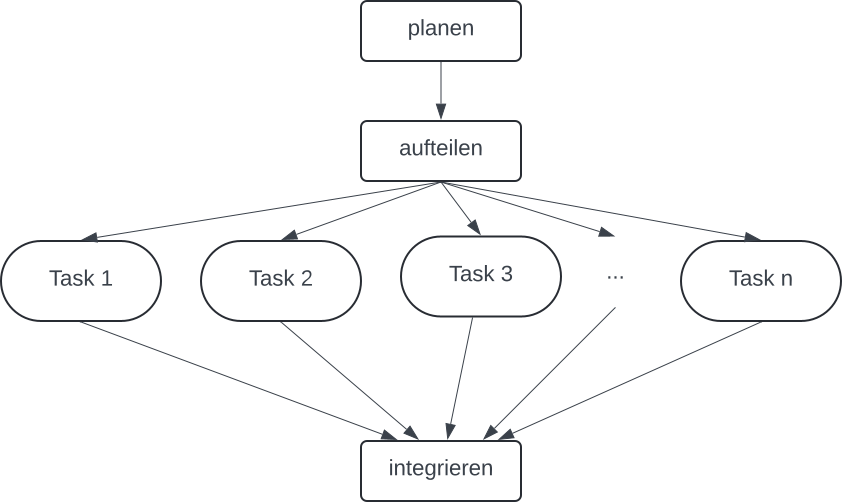
\includegraphics[scale=0.4]{chapters/Prozessmodelle/img/nebenlaeufigkeit}
    \caption{Skizze von nebenläufigem Vorgehen. (Quelle: in Anlehnung an \cite[29]{Wed09})}
    \label{fig:nebenlaeufig}
\end{figure}


\noindent
Nebenläufige Entwicklung wird meist \textit{nicht} isoliert eingesetzt, sondern i.d.R. im Zusammenhang mit agilen Verfahren.

\subsubsection*{Vorteile}

\begin{itemize}
    \item Jede Funktionalität kann nach Fertigstellung ausgeliefert werden.
    \item Probleme bei parallel bearbeiteten Aufgaben beeinflussen sich nicht gegenseitig.
\end{itemize}

\subsubsection*{Nachteile}

\begin{itemize}
    \item Management der parallelen Bearbeitung ist aufwändig, da pro Aufgabe i.d.R. mehrere Mitarbeiter beteiligt sind.
    \item Nebenläufige Entwicklung kann Kommunikation mit dem Kunden und Vertragsgestaltung erschweren.
    \item Abhängigkeit von verschiedenen Aufgaben kann problematisch werden (redundante oder unterschiedliche Implementierung derselben oder ähnlicher Anforderungen\footnote{
    s. hierzu auch den Abschnitt ``Conformist`` bei \textit{Evans} (\cite[361]{Eva03})
    }).
\end{itemize}